\documentclass{article}
\usepackage{graphicx}
\usepackage[margin=1.5cm]{geometry}
\usepackage{amsmath}

\begin{document}

\title{Monday Reading Assessment: Unit 6, Circular Motion}
\author{Prof. Jordan C. Hanson}

\maketitle

\section{Memory Bank}

\begin{itemize}
\item $\Delta s = r \Delta \theta$
\item $\omega = \frac{\Delta \theta}{\Delta t}$ ... Definition of angular velocity
\item $v = r\omega $ ... Relationship between tangential velocity and angular velocity a distance $r$ from the center
\item $C = 2\pi r$ ... Circumference of a circle, given the radius, $r$.
\end{itemize}

\begin{figure}[ht]
\centering
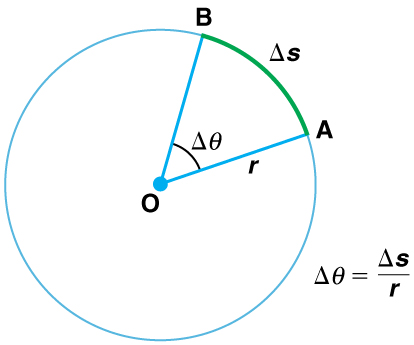
\includegraphics[width=0.3\textwidth]{circle.jpeg}
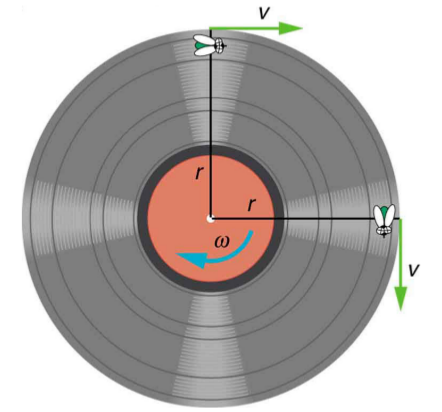
\includegraphics[width=0.25\textwidth]{record.png}
\caption{\label{fig:record} (Left) A circle with a radius $r$.  Arc length $\Delta s$ around the edge is related to the angle $\Delta \theta$.  (Right) A record that is spinning counter-clockwise.}
\end{figure}

\section{Angular Displacement and Velocity}

\begin{enumerate}
\item Suppose an object is circular, with a radius of 0.1 m. (a) What is the circumference?  Suppose we mark a point on the edge of this object, and the object begins to rotate.  The mark returns to the original location after 1.5 seconds.  (b) Divide the circumference by this time to get a speed.  (c)  If the motion is constant, how many times per minute will this object rotate? \\ \vspace{1cm}
\item Consider Fig. \ref{fig:record} (right).  A record spins at 45 revolutions per minute (rpm).  (a) How many revolutions per second is this? (b) Using a formula from the memory bank, calculate the speed of a point around the edge of the record, if $r = 0.15$ cm. (c) If the record is left playing for one hour, and continues to spin at 45 rpm, how many times will it rotate?
\end{enumerate}

\end{document}
